\subsection{Modellwahl}
Wie bereits erw\"ahnt, wurden f\"unf unterschiedliche Herangehensweisen betrachtet, um ein geeignetes Modell zu finden.

\paragraph{Wahl der Verteilung}
Wie Osgood in [Osgood2000]\footnote{Vgl.: D.Wayne Osgood: Poisson-Based Regression Analysis of Aggregate
Crime Rates, Journal of Quantitative Criminology, Vol. 16, No. 1, 2000}
schreibt, ist es von Vorteil Poissonverteilungen zu nutzen, um Kriminalit\"atsraten zu analysieren.
Poissonbasierte Regressionsmodelle sind bei Beobachtungen von Verbrechensdelikten eine gute Wahl, da sie anhand von Annahmen \"uber Fehlerverteilungen gebaut werden, die mit der Art der Ereignisanzahl konsistent sind\footnote{[Osgood2000] S.21}. \\
Osgood empfiehlt daher die Verwendung der negativen Binomialverteilung. Diese wurde von Poisson selber in den 1820-er Jahren entwickelt, um Verbrechen zu analysieren\footnote{Maltz, M. D. (1994). Operations research in studying crime and justice: Its history and accom-
plishments. In Pollock, S. M., Rothkopf, M. H., and Barnett, A. (eds.), Operations
Research and the Public Sector, Volume 6 of Handbooks in Operations Research and
Management Science, North-Holland, Amsterdam, pp. 200 - 262.}.
Daher wurde in dieser Arbeit nicht das \texttt{OLS}-Verfahren (ordinary least-squares) verwendet, welches eigentlich die Standardmethode in solchen Untersuchungen ist. \\
Eine Normalverteilung oder eine symmetrische Fehlerverteilung kann hier nicht angenommen werden, da die Verbrechensanzahl sehr gering sein kann.
Die kleinstm\"ogliche Anzahl an Verbrechen in einem County ist Null.
Daher m\"usste eine Fehlerverteilung immer mehr verzerrt werden\footnote{Vgl.: [Osgood2000] S. 21 f.}.
In Abbildung \ref{fig:nbd} sind 100 Zufallszahlen auf Basis der negativen Binomialverteilung mit $\theta = 0.7$ dargestellt.

\begin{figure}
\centering
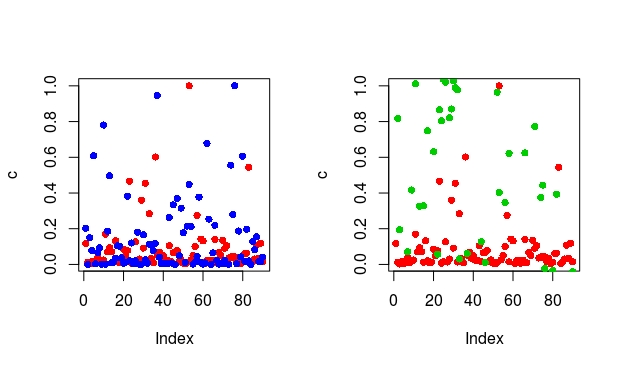
\includegraphics[scale=0.7]{./jpgs/rnegbin.jpeg}
\caption{In beiden Diagrammen sind die relativierten Verbrechenszahlen rot dargestellt.
		 In dem linken Diagramm wurden dazu in blau mit Hilfe von \texttt{rnegbin()} berechnete     Zufallszahlen hinzugef\"ugt.
		 Das rechte Diagramm enth\"alt stattdessen zus\"atzlich Zufallszahlen, die mit \texttt{rnorm()} berechnet wurden.}
\label{fig:nbd}
\end{figure}
\par\smallskip

Um die Annahme der negativen Binomialverteilung zu rechtfertigen wurden zu Beginn der Arbeit zwei Modelle verglichen, welche die selben Daten und die selbe Formel nutzen, aber unterschiedliche Verteilungen annehmen.
Es wurde der gesamte Datensatz von allen 90 Counties genutzt.
Die verwendete Formel war:
\begin{equation}
crimes = \beta_0 \cdot prbarr:prbpris + \beta_1
\end{equation}

Un zu entscheiden, welches der Modelle besser sch\"atzt, wurden die Akaike-Werte der beiden Modelle miteinander verglichen.
In Tabelle \ref{tab:agn} finden sich diese Zahlen wieder.
Der Akaikewert von Modell \textsc{m1Nb} ist wesentlich geringer als der von \tesxtsc{m1}.
Dies sagt eigentlich nicht aus, dass \textsc{m1Nb} ein besseres Modell als \textsc{m1} ist.
Vor allem aber ist die Devienz des ersten Modells viel gr\"o\ss{}er, als die des binomialverteilten.
Dies spricht f\"ur eine deutliche Verbesserung.
\par\smallskip
W\"ahrend der Untersuchung wurden nat\"urlich mehrere Gleichungen angenommen als diese eine.
Die Ergebnisse haben aber alle zu diesem selben Schluss gef\"uhrt.
Eine graphische Veranschaulichung der Gegen\"uberstellung der beiden Verteilungen findet sich in Abbildung \ref{fig:nbd}.
Hier sieht man recht gut, dass die Verbrechenszahlen eher zu einer negativen Binomialverteilung passen, als zu einer normalen Gau\ss{}verteilung.
  
\begin{table}[ht]
\centering
\begin{tabular}{rrrr}
  \hline
 	   & df & AIC & Devienz\\ 
  \hline
	m1 & 3.00 & 1789.10 & 2118963611\\ 
  m1Nb & 3.00 & 1598.57 & 106.3874\\ 
   \hline
\end{tabular}
\caption{Gegen\"uberstellung der Akaike-Werte zweier Modelle. m1 nimmt eine Gau\ss{}verteilung an, w\"ahrend m1Nb eine negative Binomialverteilung annimmt.}
\label{tab:agn}
\end{table}


\label{sec:preg}
\paragraph{Die besondere Rolle von der Einflussgr\"o\ss{}e \textit{region}}
Bei der Einflussgr\"o\ss{}e \textit{region} handelt es sich um eine dichotome Dummy-Variable.
Sie gibt an in welchem Bereich des Bundesstaates (= die Region) sich das County befindet.
Es gibt drei m\"ogliche Werte, welche diese Variable annehmen kann: \textit{central}, \textit{west} und \textit{other}.

\begin{figure}
\centering
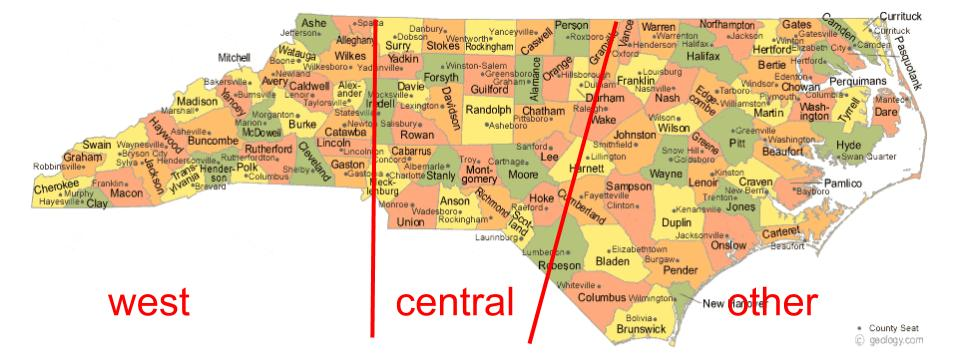
\includegraphics[scale=0.7, keepaspectratio,width=\textwidth,height=\textheight]{./jpgs/ncc.jpg}
\caption{Diese \"Ubersicht zeigt in etwa an wo sich die drei unterschiedlichen Regionen befinden
\footnote{https://geology.com/county-map/north-carolina.shtml, 28.03.18, 10:57} }
\label{fig:ncc}
\end{figure}

Anhand von Abbildung \ref{fig:ncc} sieht man, \"uber welche Bereiche des Bundesstaates sich diese drei Regionen erstrecken. \\
Bei der Untersuchung dieser Einflussgr\"o\ss{}e ist aufgefallen, dass diese Variable wohl hinzugef\"ugt wurde, um die st\"arker besiedelten Regionen des Bundesstaates zu kennzeichnen.
So sind die Counties, die sich z.B in der Region \textit{central} befinden wesentlich st\"arker bev\"olkert, als die Counties in der Region \textit{west}.
Die Region \textit{other} ist fl\"achenm\"a\ss{}ig die gr\"o\ss{}te, ihre Counties haben aber trotzdem eine gr\"o\ss{}ere Bev\"olkerungsdichte als die Counties der kleinsten Region \textit{west}.
Daher handelt es sich bei \textit{west} wohl auch um eine st\"arker besiedelte Region.
Dies ist deswegen interessant zu betrachten, da schon sehr fr\"uh in den Untersuchungen aufgefallen ist, dass die Variable \textit{density} sehr gut dazu geeignet ist, ein gutes Modell zu finden.

\begin{table}[ht]
\centering
\begin{tabular}{cccccc}
  \hline
  \textit{region} & Anzahl Counties & Durchschnitt \textit{crimes} & Median \textit{crimes} & \diameter \textit{density} \\ 
  \hline
    central & 34 & 4764 & 2172 & 196\\
	west & 21 & 1027 & 513  & 86\\ 
  	other & 35 & 2250 & 1235 & 101\\ 
   \hline
\end{tabular}
\caption{Vergleich der durchschnittlichen Eigenschaften der Counties aus den jeweiligen Regionen.}
\label{tab:cvp}
\end{table}

In Tabelle \ref{tab:cvp} befindet sich eine Gegen\"uberstellung der durchschnittlichen Werte von der Zielgr\"o\ss{}e \textit{crimes} und der durchschnittlichen Bev\"olkerungsdichte (\textit{density}) der drei Regionen.
Bei der Betrachtung wird ersichtlich, dass es scheinbar einen Zusammenhang zwischen \textit{region} und \textit{density} gibt.
In l\"andlichen Gegenden sind die \textit{crimes}-Werte geringer.
Befindet sich in dieser l\"andlichen Gegend aber eine gr\"o\ss{}ere Stadt, ist \textit{crimes} auch erh\"oht.

\begin{figure}
\centering
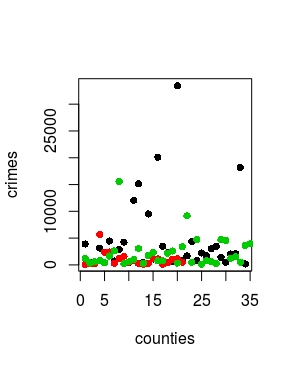
\includegraphics[scale=0.7]{./jpgs/regionc.jpeg}
 \abovecaptionskip
\caption{Anhand der Farbgebung l\"asst sich erkennen, in welchen Regionen die Counties wieviele Verbrechen gemeldet haben. Schwarz sind Counties aus der Region \textit{central}, rot die Counties aus der Region \textit{west} und gr\"un die Counties aus der Region \textit{other}.}
\label{fig:rc}
\end{figure}

\begin{figure}
\centering
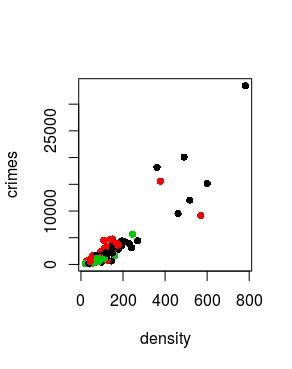
\includegraphics[scale=0.7]{./jpgs/cdc.jpeg}
 \abovecaptionskip
\caption{Hier wird das Ver\"altnis \textit{density} zu \textit{crimes} dargestellt.}
\label{fig:cdc}
\end{figure}


In Abbildung \ref{fig:rc} wird ersichtlich, dass es in der Region \textit{central} einige Counties gibt, die wesentlich mehr Delikte gemeldet haben, als die Counties aus anderen Regionen.
Dies scheint an der h\"oheren Bev\"olkerungsdichte \textit{density} zu liegen, wie die Darstellung \ref{fig:cdc} aufzeigt. \\
Tats\"achlich wird sich herausstellen, dass diese Wechselwirkung zwischen \textit{region} und \textit{density} (also \textit{density:region}) Bestandteil von vielen guten Modellen sein wird.
Daher wurde diese Dummy-Variable nicht weiter ver\"andert.
\textsf{R} behandelt solche Variablen automatisch mithilfe von \texttt{as.factor()} als diskrete Zahlen.


\paragraph{Herangehensweisen}
\subparagraph{explorative Herangehensweise}
Um ein gutes Gef\"uhl f\"ur die Merkmalsvektoren zu bekommen, wurden zun\"achst einige Modelle ausprobiert und mittels AIC verglichen.
Damit ein Vergleichswert nach dem Akaike-Ma\ss{} vorhanden war, wurde ein komplettes Modell angenommen, das aus allen vorhandenen Merkmalen besteht. Dieses Modell hei\ss{}t \textit{mAll}. Die entsprechende Formel sieht so aus:
\begin{equation}
crimes = prbarr+prbpris+polpc+density+area+taxpc+region+pctmin+pctymale+wcon+wsta+wser+wtrd+wfir
\end{equation}
Es wurde bewusst darauf verzichtet in diesem 'gesamten' Modell die Intersections (Wechselwirkungen) der einzelnen Merkmale zu betrachten. Grund daf\"ur ist, dass das Akaike-Ma\ss{} Modelle mit vielen Einflussgr\"o\ss{}en mehr bestraft, als solche die weniger besitzen. Da bei dieser Untersuchung das Akaike-Ma\ss{} das am h\"aufigsten verwendete Kriterium war, sollte also das erste Modell, mit dem die anderen verglichen wurden, nicht einen gro\ss{}en negativen Wert aufweisen, so wie das in diesem Fall der Fall gewesen w\"are. (Der Akaike-Wert des Modells, das alle Merkmale und alle Wechselwirkungen zwischen diesen betrachtet, betr\"agt -3441.465. In diesem Modell gibt es 91 Freiheitsgrade.)
Die Daten \texttt{crimes.data}, welche der Funktion \texttt{glm.nb(formula, data = crimes.data)} w\"ahrend der gesamten Untersuchung gegeben wurden, wurden nicht ver\"andert. Es handelt sich hierbei immer um den gesamten Datensatz aus der Datei \textit{crimes.csv}.

Im Folgenden wurde bemerkt, dass diese Merkmale durchaus gruppiert betrachtet werden k\"onnen. Daher bestand die erste Idee darin, die unterschiedlichen Gruppierungen je Modell zu betrachten:
Die ersten beiden Merkmale (\textit{prbarr} und \textit{prbpris}) geben beide Verh\"altnisse zum Anteil aller Straft\"ater in einem County an. Daher wurde ein Modell aus diesen beiden Einflussgr\"o\ss{}en betrachtet.
\begin{equation}
crimes = prbarr:prbpris
\end{equation}
Die Einflussgr\"o\ss{}en \textit{density} und \textit{area} sind beides r\"aumliche Merkmale. Auch sie wurden in einem Modell zusammengefasst. Wie in \ref{sec:preg}
% wie ging das nochmal mit den referenzieren auf einen anderen bereich? *seufz...

\subparagraph{Vergleich aller Modelle mit jeweils nur einem Merkmal}
\subparagraph{Verwendung von step() und anschließende Minimierung des Modells}
\subparagraph{strukturierte Suche nach einem geeigneten Modell}
\subparagraph{Verwendung von cor()}
\subparagraph{Die Gewinnermodelle}

\newpage 
\subsection{Simulationsaufgabe}
\paragraph{Beschreibung simulation()}
\paragraph{Auswertung der Ergebnisse}
\subparagraph{einfaches Modell: \textit{mDensity}}
\subparagraph{Ergebnisse mit Gewinnermodell aus der ersten Aufgabe}
Hier leite ich zur Diskussion \"uber.